\documentclass[letterpaper]{article} % DO NOT CHANGE THIS
\usepackage[submission]{aaai2027}  % DO NOT CHANGE THIS
\usepackage[hyphens]{url}  % DO NOT CHANGE THIS
\usepackage{graphicx} % DO NOT CHANGE THIS
\urlstyle{rm} % DO NOT CHANGE THIS
\def\UrlFont{\rm}  % DO NOT CHANGE THIS
\usepackage{natbib}  % DO NOT CHANGE THIS AND DO NOT ADD ANY OPTIONS TO IT
\usepackage{caption} % DO NOT CHANGE THIS AND DO NOT ADD ANY OPTIONS TO IT
\frenchspacing  % DO NOT CHANGE THIS
\usepackage{booktabs}
\usepackage{xcolor}
\pdfinfo{
/TemplateVersion (2027.1)
}
\setcounter{secnumdepth}{0}

% ---- every number comes from code/make_finfm_tables.py; never type a result by hand ----
\newcommand{\ConfNHidden}{2,570}
\newcommand{\ConfNShown}{2,570}
\newcommand{\ConfRaisedHidden}{10}
\newcommand{\ConfRaisedShown}{92}
\newcommand{\KeptAgent}{2.1}
\newcommand{\KeptBlock}{6.8}
\newcommand{\KeptRepair}{80.4}
\newcommand{\NBundles}{1,900}
\newcommand{\NPersona}{22,800}
\newcommand{\PersonaViol}{53.8}
\newcommand{\RiskMgrKeptOrigFive}{5.5}
\newcommand{\RiskMgrKeptOrigFourO}{0.0}
\newcommand{\RiskMgrKeptOrigFourOne}{0.1}
\newcommand{\RiskMgrKeptRepairFirstFive}{23.0}
\newcommand{\RiskMgrKeptRepairFirstFourO}{52.6}
\newcommand{\RiskMgrKeptRepairFirstFourOne}{52.8}
\newcommand{\VetoRate}{93}


\title{Fix What Is Checked, Inflate What Is Not:\\How LLM Trading Agents Respond to Investor-Mandate Enforcement}
\author{Anonymous Submission}
\affiliations{}

\begin{document}
\maketitle

\begin{abstract}
LLM trading agents are increasingly wrapped in rule layers that enforce an investor's mandate, but these layers are judged by their violation rate alone. We compare four ways of enforcing a mandate on the \emph{same} LLM trade proposals and score each on what the trade would have earned: blocking the trade, an LLM risk manager, deterministic repair, and feeding the rule engine's rejection reasons back to the model. Using \NBundles{} point-in-time evidence bundles for 100 US and Indian (NSE) large caps, all dated after the three decision models' training cutoffs, we find three things. A text persona produces mandate-blind sizing: \PersonaViol\% of decisions exceed the position cap. Blocking and an LLM risk manager reach full compliance by abstaining, keeping \KeptBlock\% and \KeptAgent\% of proposed trades, while deterministic repair keeps \KeptRepair\%. Given the engine's reasons, models repair the clauses the engine can check (size, stop) and \emph{raise their stated confidence to the required bar} in \ConfRaisedShown\% of cases without any new evidence, versus \ConfRaisedHidden\% when the bar is not mentioned. This shows that enforcing a numerical threshold on self-reported confidence need not enforce the intended reliability requirement. We argue that enforcement should be evaluated on participation and realised risk, not compliance alone, and that gates must sit on quantities that code computes.
\end{abstract}

% =====================================================================================
\section{Introduction}
Multi-agent LLM trading systems give language models the whole trade: analyst agents read data, a trader proposes direction, size and exits, and a risk-manager agent reviews it \citep{xiao2024tradingagents,yu2024fincon,zhang2024finagent}. Recent work keeps the LLM but wraps it in deterministic code that caps, clips or vetoes its proposals \citep{cai2026openpm,kukreja2026biasmix,qu2026clqt}. These guardrails are reported by how often they leave a violation, a number that every guardrail can drive to zero by refusing to trade.

We ask a different question: \emph{when a mandate is enforced on an LLM agent, what does the agent end up doing, and what does that do to the trade?} We hold one set of LLM proposals fixed and apply four enforcement mechanisms to it after the fact, so every comparison is paired. Our contributions:
\begin{itemize}
\item A paired comparison of four enforcement mechanisms on \NPersona{} post-cutoff LLM trade decisions in two equity markets, scored on compliance, participation and realised, cost-adjusted outcome.
\item Evidence that rejection-style enforcement (blocking, an LLM risk manager) buys compliance by abstention, while deterministic repair keeps most trades and halves P\&L dispersion.
\item A controlled test of feedback-based enforcement: the agent fixes verifiable clauses and inflates the one it self-reports, which we isolate with a control that withholds the confidence clause.
\end{itemize}
For a deployed system, a mandate is an operational constraint: a plausible forecast does not justify exceeding a position cap.

% =====================================================================================
\section{Related Work}
TradingAgents, FinCon and FinAgent organize language models into financial decision workflows \citep{xiao2024tradingagents,yu2024fincon,zhang2024finagent}. Their apparent returns depend on evaluation design: StockBench and FINSABER test broader market conditions and emphasize comparison with simple baselines, while look-ahead studies identify historical contamination risks \citep{chen2025stockbench,li2025finsaber,gao2025lookahead}. We therefore evaluate enforcement on fixed proposals rather than claim a profitable strategy.

OpenPM translates investor mandates into portfolio constraints and projects allocations; BiasMix-Finance repairs generated allocations through convex projection \citep{cai2026openpm,kukreja2026biasmix}. CLQT links risk discipline to its constrained pipeline, while noting that the constraint layer is not separately ablated \citep{qu2026clqt}. Inside the Trading Loop assigns portfolio construction to explicit rules \citep{tradingloop2026}. Closest to our feedback experiment, TradeArena compares true, placebo and hidden risk reports and measures subsequent intended exposure \citep{xue2026tradearena}. Our narrower question is whether per-decision rejection reasons change the self-reported confidence being gated, with the underlying market evidence fixed.

Verbalized confidence can be miscalibrated \citep{xiong2024uncertainty}; financial confidence must also be interpreted relative to the decision rule using it \citep{singh2026ordinal}. Sycophancy and intrinsic self-correction studies show that revisions need not improve correctness \citep{sharma2024sycophancy,huang2024selfcorrect}. Reward-hacking theory distinguishes success on a proxy from the intended objective \citep{skalse2022rewardhacking}. We test that distinction in mandate enforcement, without attributing deliberate deception to the model.

% =====================================================================================
\section{Setup}
\paragraph{System.} Five specialist agents (technical, news, fundamental and macro LLM judges, and a logistic-regression price model) turn point-in-time data into evidence items with a direction in $[-1,1]$ and a confidence in $[0,1]$. An investor profile (Table~\ref{tab:profiles}) sets a position cap, a stop-loss, a confidence bar and which agents to consult. A deterministic risk engine checks every decision against the profile and returns APPROVED or VETOED with written reasons (clause, value, limit). The policy router chooses which frozen evidence items each profile sees; those items are identical across enforcement arms. Appendix Figure~\ref{fig:architecture} summarizes the pipeline.

\paragraph{Data and models.} We rebuild every agent as of 19 monthly decision dates (Jan 2025--Jul 2026) for 50 US and 50 NSE large caps, using only information available before the next session's open (\NBundles{} bundles). Three decision models (gpt-4o-mini, gpt-4.1-mini, gpt-5-mini) have published training cutoffs before every decision date. Each model receives the bundle and a profile, either as a short text persona or with the numeric limits stated, and proposes action, size, stop, target and its confidence. The evidence model is fixed to gpt-4o-mini; evidence is reused rather than regenerated during decision-model comparisons. A separate exploratory local-model check uses one randomly selected bundle per month and market (38 bundles, all four profiles), fixed with seed 20261123 before comparing outcomes; Appendix Table~\ref{tab:local} reports it separately.

\paragraph{Enforcement arms.} All arms start from the same persona proposal $U$:
(i) \emph{Block}: if the engine vetoes $U$, WAIT.
(ii) \emph{LLM risk manager}: a second LLM sees $U$ and the numeric mandate and may approve, modify or reject.
(iii) \emph{Repair}: WAIT if confidence is below the bar; otherwise clip size to the cap and tighten the stop to the policy's.
(iv) \emph{Feedback}: the same model sees its proposal and the engine's reasons and revises, for up to three rounds; a still-vetoed revision becomes WAIT.
As a control for (iv), \emph{feedback without the confidence clause} gives the model only the size and stop reasons while the engine still enforces the bar.

\paragraph{Outcomes.} A decision taken at the close of day $t$ enters at the next open and is held for the profile's horizon (1, 5, 20 or 40 days), with stops and targets checked on daily highs and lows and round-trip costs of 14 bp (US) and 36 bp (NSE). Utility is the position-weighted net return in basis points of equity; WAIT is 0. Intervals are 95\% bootstraps over decision months. The outcome rule was fixed before any LLM outcome was computed. The outcome specification is recorded in a repository amendment dated 12 October 2026; this is a dated protocol, not a public preregistration.

% =====================================================================================
\section{Results}
\begin{table*}[t]
\centering
\footnotesize
\begin{tabular}{lrrrrrrrl}
\toprule
Pipeline & Viol.\,\% & Trades\,\% & Kept\,\% & Exp./cap & Aggr./Cons. & SD & CVaR$_5$ & Mean P\&L [95\% CI] \\
\midrule
Raw persona proposal & 53.8 & 74.4 & -- & 1.55 & 1.4 & 53.7 & -88.8 & -0.93 [-1.75, -0.14] \\
Block (veto $\to$ WAIT) & 0.0 & 5.1 & 6.8 & 0.05 & -- & 5.5 & -0.4 & -0.07 [-0.18, +0.03] \\
LLM risk manager & 0.0 & 1.6 & 2.1 & 0.01 & -- & 1.5 & -0.1 & -0.02 [-0.04, -0.01] \\
Deterministic repair & 0.0 & 59.8 & 80.4 & 0.59 & 8.2 & 22.2 & -50.3 & -0.19 [-0.54, +0.14] \\
Limits stated in prompt & 0.0 & 47.0 & -- & 0.41 & 10.9 & 17.5 & -37.6 & -0.20 [-0.58, +0.11] \\
Code only & 0.0 & 40.1 & -- & 0.39 & 14.5 & 18.7 & -47.9 & -0.09 [-0.59, +0.35] \\
\bottomrule
\end{tabular}

\caption{Enforcement on text-persona proposals (\NPersona{} decisions, three models pooled, primary window). Viol.: executed size above the profile cap. Kept: share of the LLM's proposed trades still executed. Exp./cap: mean position over the cap (WAIT = 0). Aggr./Cons.: mean aggressive-profile position over mean conservative-profile position on the same bundles (the mandate implies 4.0). SD, CVaR$_5$ and mean are decision P\&L in bp of equity, net of costs. ``Limits stated in prompt'' and ``Code only'' are separate decisions on the same bundles, shown for reference.}
\label{tab:enforcement}
\end{table*}

\paragraph{Personas produce mandate-blind sizing.} \PersonaViol\% of persona decisions exceed the position cap, and the engine vetoes \VetoRate\% of proposed trades. Table~\ref{tab:enforcement} shows that aggressive and conservative profiles receive much less differentiated sizing than their caps imply. Explicit numerical limits remove position-cap violations in this sample.

\paragraph{Rejection buys compliance by abstention.} Blocking keeps \KeptBlock\% of proposed trades and the standard-prompt LLM risk manager keeps \KeptAgent\%, despite being allowed to resize. A repair-first reviewer prompt retains \RiskMgrKeptRepairFirstFourO\%, \RiskMgrKeptRepairFirstFourOne\% and \RiskMgrKeptRepairFirstFive\% for proposals from gpt-4o-mini, gpt-4.1-mini and gpt-5-mini, respectively. Thus abstention is sensitive to the reviewer prompt, not an inevitable property of LLM review. Deterministic repair keeps \KeptRepair\% and lowers decision-level dispersion and tail losses (Table~\ref{tab:enforcement}). Its compliance is guaranteed by construction, and reduced exposure itself reduces risk: this is evidence for compliant participation, not improved forecasting or superior returns.

\begin{table*}[t]
\centering
\footnotesize
\setlength{\tabcolsep}{3pt}
\begin{tabular}{lrrrr}
\toprule
 & & \multicolumn{2}{c}{Raised to bar (\%)} & Kept (\%) \\
Model & $n$ & bar shown & bar hidden & bar shown \\
\midrule
gpt-4o-mini & 568 & 65.8 [61, 70] & 0.5 [0, 2] & 65.1 \\
gpt-4.1-mini & 332 & 94.0 [90, 97] & 0.9 [0, 3] & 93.7 \\
gpt-5-mini & 1670 & 99.9 [99, 100] & 14.6 [12, 17] & 95.5 \\
\bottomrule
\end{tabular}

\caption{Feedback on proposals vetoed for low confidence \emph{and} for size or stop. ``Bar shown'': the feedback lists every violated clause. ``Bar hidden'': the same feedback without the confidence clause, which the engine still enforces. No new evidence is given in either arm. Brackets: 95\% Wilson intervals.}
\label{tab:confidence}
\end{table*}

\paragraph{Feedback: fix what is checked, inflate what is not.} With all rejection reasons shown, models raise stated confidence to the bar in \ConfRaisedShown\% of eligible cases ($n=\ConfNShown$), versus \ConfRaisedHidden\% when the confidence clause is hidden ($n=\ConfNHidden$; Table~\ref{tab:confidence}). Both groups also violate size or stop rules, so each receives a reason to revise. No new market evidence is supplied. The contrast shows sensitivity of the reported confidence to the gate; it does not establish a change in predictive information. In an exploratory profile-by-region standardized comparison, confidence-raised gpt-5-mini trades have lower hit rate and net decision P\&L than originally above-bar trades, while the other two models have intervals spanning zero (Appendix Table~\ref{tab:matched}). This observational comparison does not identify a causal effect of raising confidence.

% =====================================================================================
\section{Discussion and Limitations}
\paragraph{Design rules.} (1) Give the agent the mandate as numbers. (2) Repair rather than refuse, and report participation and risk at matched exposure next to compliance. (3) Never gate on a quantity the agent reports about itself; gate on quantities code computes from the evidence.
\paragraph{Limitations.} Our evidence signals are weak, so we make no return or deployability claim. The primary study covers nineteen months, three decision models from one provider, and one fixed evidence model. Current large-cap membership introduces survivorship bias. A fixed fiscal-year reporting lag approximates actual disclosure availability; post-cutoff dates do not prove absence of all contamination. Each decision starts from a flat portfolio, so we do not evaluate interacting positions, turnover or portfolio-level capital constraints. Daily bars approximate execution, and the intraday-named profile uses a one-session horizon. Confidence is a model report rather than a verified probability. Feedback can change direction and size as well as confidence; the matched analysis remains observational. The dated outcome amendment is not a public preregistration. Additional open-weight experiments do not eliminate model, provider or quantization dependence.

\bibliography{refs}

\appendix
\section{Protocol and supplementary analysis}
\begin{table}[h]
\centering
\begin{tabular}{lrrrr}
\toprule
Profile & Cap & Stop & Bar & Horizon \\
\midrule
aggressive growth & 8 & 5 & 0.6 & 5 \\
conservative & 2 & 3 & 0.75 & 20 \\
intraday & 4 & 1.5 & 0.65 & 1 \\
long term & 5 & 12 & 0.7 & 40 \\
\bottomrule
\end{tabular}

\caption{Investor profiles. Size and stop are percentages; the confidence bar is a unitless threshold. Horizons are trading sessions.}
\label{tab:profiles}
\end{table}

\begin{figure}[h]
\centering
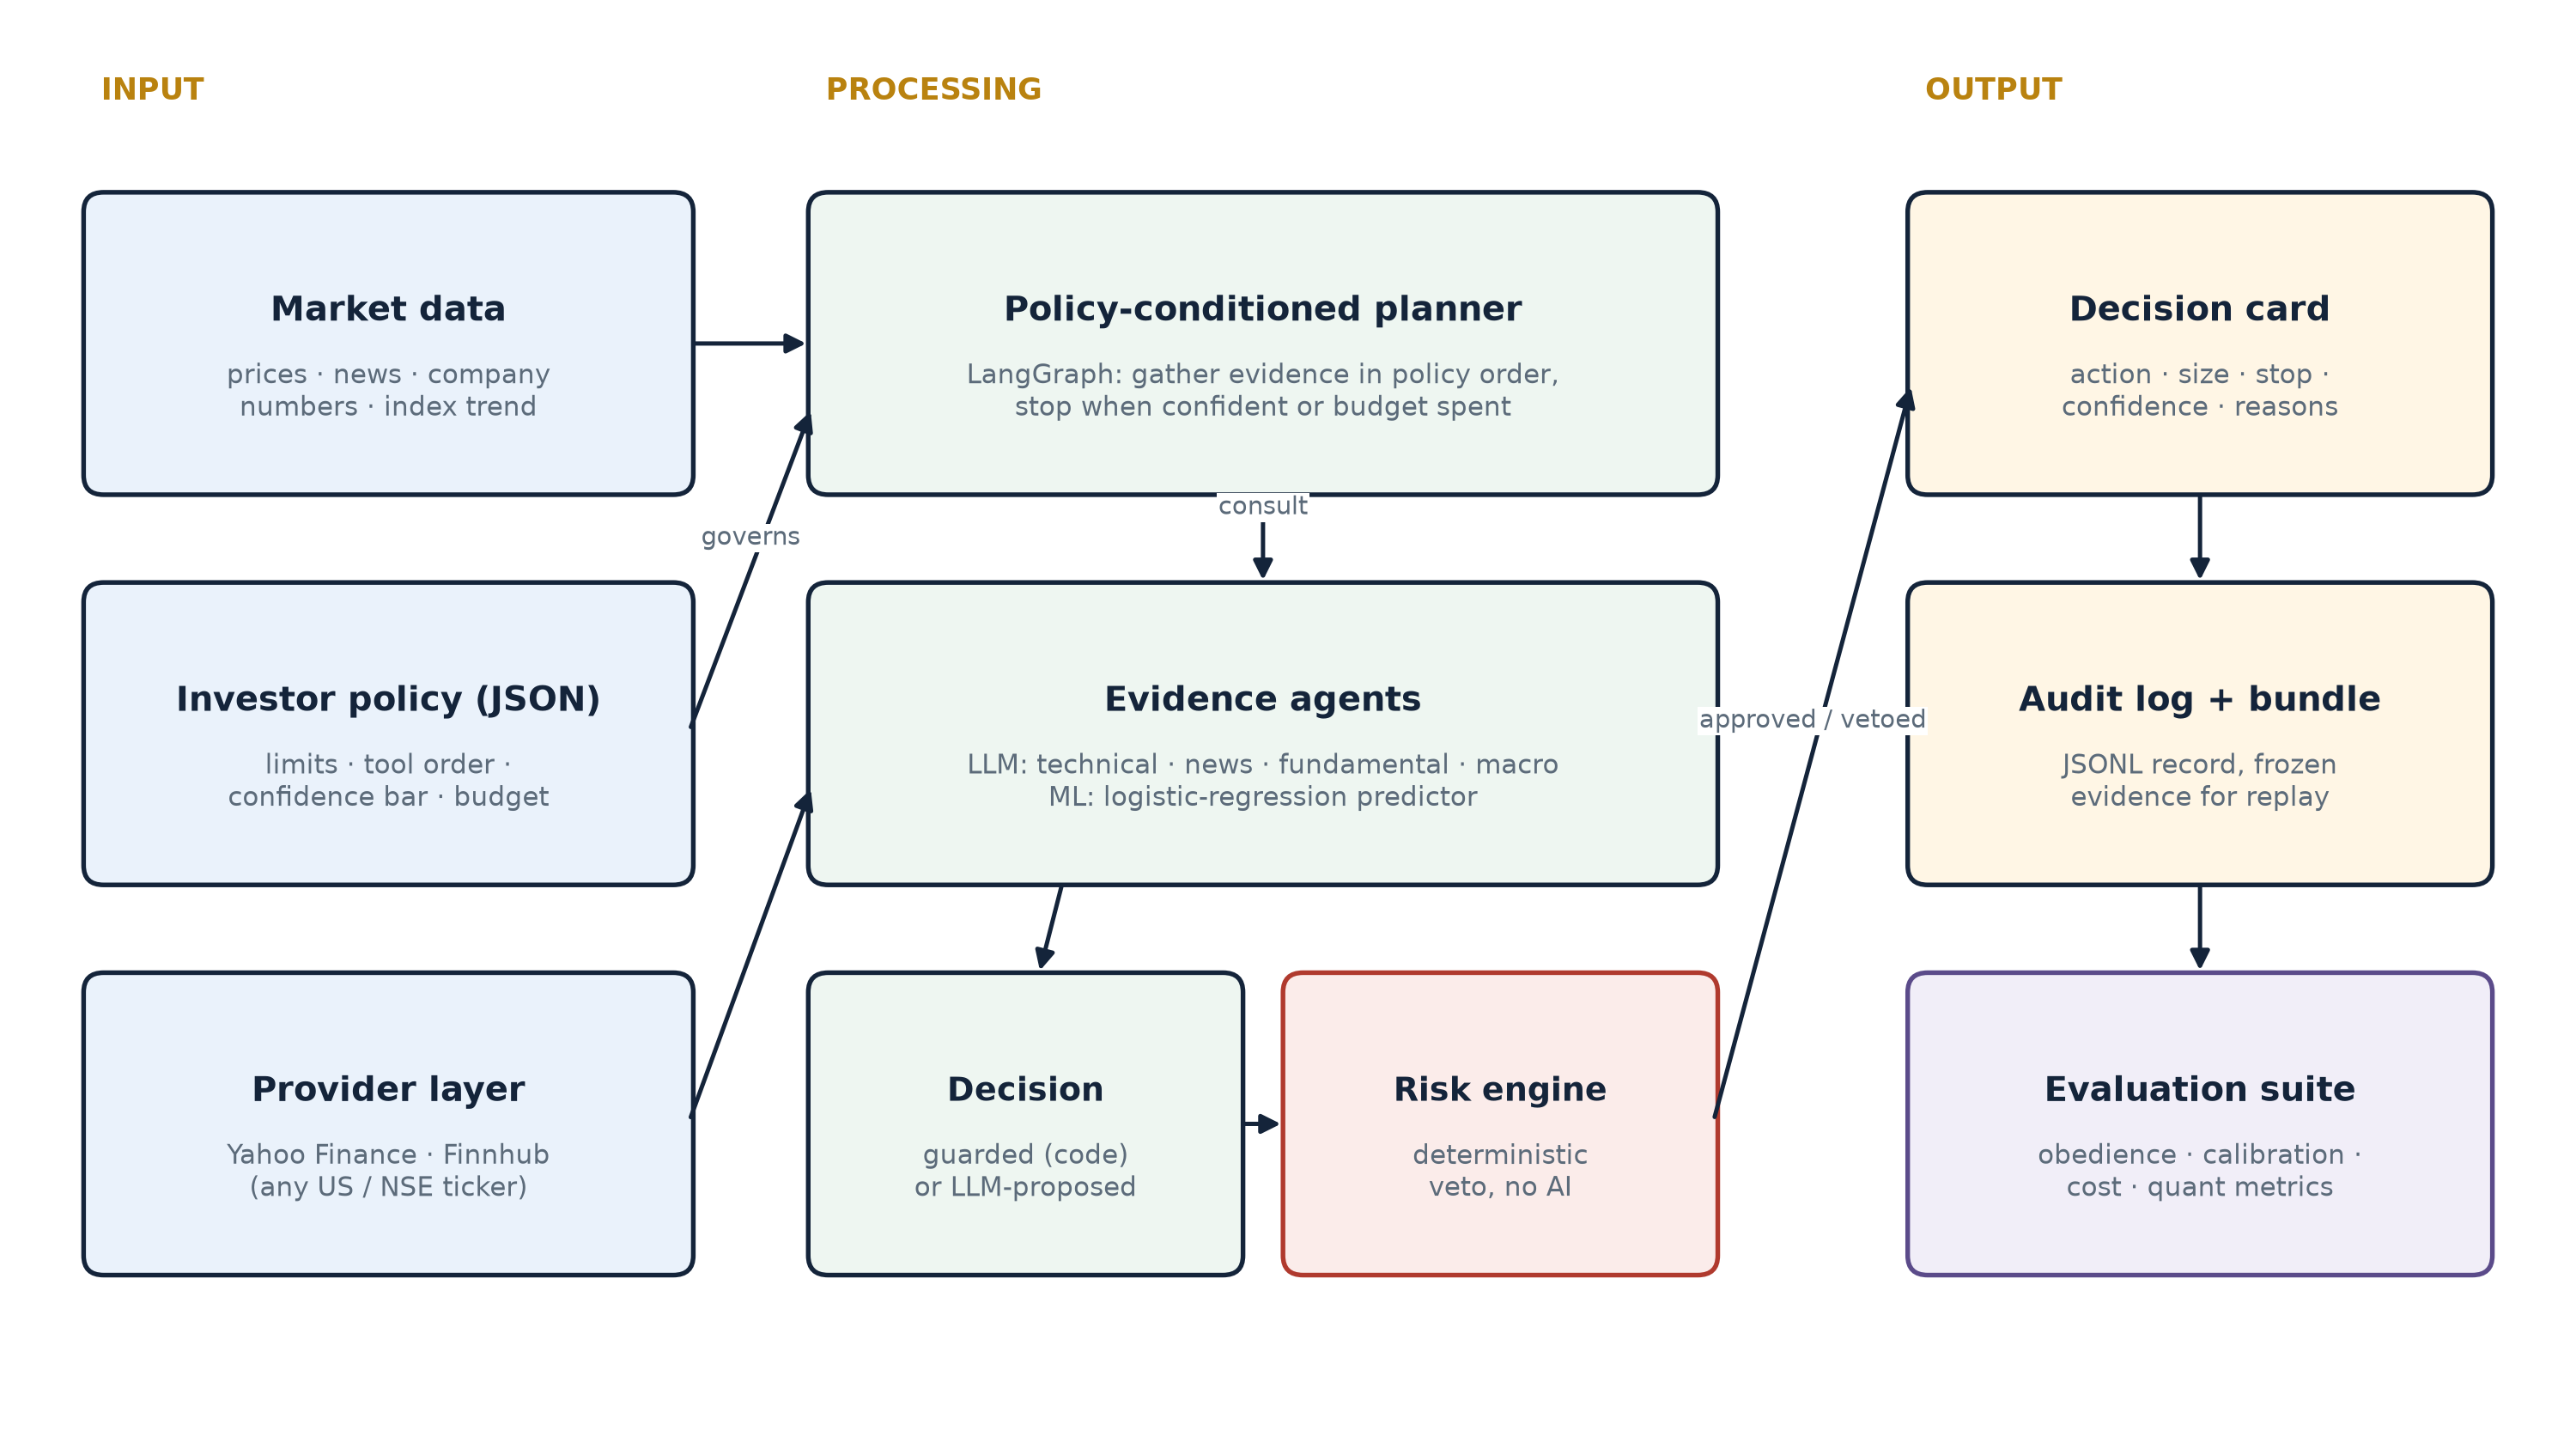
\includegraphics[width=\columnwidth]{figures/architecture.png}
\caption{Evidence, decision and deterministic enforcement pipeline.}
\label{fig:architecture}
\end{figure}

\begin{table*}[t]
\centering
\begin{tabular}{lrrll}
\toprule
Model & Raised & Above & Hit difference (pp) & P\&L difference (bp) \\
\midrule
gpt-4o-mini & 371 & 676 & +3.98 [-3.35, +11.34] & -0.88 [-3.99, +1.89] \\
gpt-4.1-mini & 329 & 744 & +3.10 [-6.40, +13.05] & -0.62 [-5.30, +3.81] \\
gpt-5-mini & 2264 & 407 & -10.64 [-15.79, -5.69] & -5.16 [-8.44, -1.73] \\
\bottomrule
\end{tabular}

\caption{Exploratory comparison of kept feedback trades: confidence-raised minus originally above-bar. Within each profile $\times$ region cell containing both groups, differences are weighted by the combined cell size. Intervals use 2,000 joint decision-month bootstrap resamples. Hit rate uses positive net trade return; P\&L is in basis points of equity. Selection, direction and position size may still differ.}
\label{tab:matched}
\end{table*}


\section{Exploratory local-model robustness}
We evaluate Llama 3.1 8B, GPT-OSS 20B, Gemma 3 4B and Phi-4 14B on the same 38 bundles (152 decisions per model), with all nineteen months and both markets represented. Published training cutoffs are December 2023, June 2024, August 2024 and June 2024, respectively. All inference uses Ollama 0.40.17 on a single laptop GPU; Llama, Gemma and Phi use Q4\_K\_M weights and GPT-OSS uses MXFP4. We use temperature zero, an 8,192-token context and a 2,048-token generation ceiling; GPT-OSS uses low reasoning effort. Model digests and environment details accompany the private experiment records.

Only proposals violating confidence and at least one size/stop clause enter the paired feedback comparison, matching the primary table's eligibility rule. All four models show a higher observed threshold-crossing rate when the confidence clause is shown, but eligible samples are small and individual Wilson intervals are wide. These are descriptive pilot results, not full-universe replications or estimates pooled with the primary models. Quantization and inference-provider differences also limit cross-model attribution. Incomplete hosted runs and the canceled full local run are excluded.

\begin{table*}[t]
\centering
\begin{tabular}{lrll}
\toprule
Model & Eligible $n$ & Bar shown (\%) & Bar hidden (\%) \\
\midrule
Llama 3.1 8B & 12 & 100.0 [75.7, 100.0] & 8.3 [1.5, 35.4] \\
GPT-OSS 20B & 25 & 64.0 [44.5, 79.8] & 24.0 [11.5, 43.4] \\
Gemma 3 4B & 20 & 25.0 [11.2, 46.9] & 10.0 [2.8, 30.1] \\
Phi-4 14B & 9 & 55.6 [26.7, 81.1] & 33.3 [12.1, 64.6] \\
\bottomrule
\end{tabular}

\caption{Exploratory local models: percentage raising confidence to the bar, with 95\% Wilson intervals. Eligible $n$ is the same in both arms for each model. Each model first produces 152 decisions on the same stratified set of 38 bundles.}
\label{tab:local}
\end{table*}

\end{document}
